\documentclass[article,12pt,twocolumn]{IEEEtran}
\usepackage[utf8]{inputenc}
\usepackage{amssymb}
\usepackage{amsmath}
\usepackage{graphicx}
\usepackage[center]{caption}
\graphicspath{{figs/}}
\title{AI1110 assignment1(ICSE Class 10 2017)}
\author{Bhargava Ram Rajulapati, CS21BTECH11052}

\begin{document}
  \maketitle
  \section*{Question 6(b)}
   A conical tent is to accommodate 77 persons.Each person must  
   have $16m^3$ of air to breathe.Given the radius of the tent as
   $7m$ find the height of the tent and also its curved surface
   area.\\
  \section*{Solution:}
  Given a conical tent which can accommodate 77 persons and each         
   person must have $16m^3$ of air to breathe.\\
  so the volume of conical tent is,
  \begin{align}
    v = 77 \times 16 m^3 \\
    v = 1232 m^3  
  \end{align}
   \begin{table}[ht!]
     \centering
     \begin{tabular}{|c|c|c|c|}
    \hline
     Symbol & formula & Value & Description \\
    \hline \hline
     $r$ & - & $7m$ & radius of the tent\\
    \hline
     $v$ & $\frac{\pi r^2 h}{3}$ & $1232 m^3$ & volume of the tent \\
    \hline
     $h$ & $\frac{3 v}{\pi r^2}$ & $?$ & height of the tent  \\
    \hline
     $s$ & $ \pi r l $ & $?$ & curved surface area \\
    \hline
 \end{tabular}
    \caption{}
    \label{table:Table1}
  \end{table} \\
  we know that volume of conical tent is same as a cone having
  radius $r$,height $h$,
  \begin{align}
     v = \frac{\pi r^2 h}{3} 
  \end{align}
  from the question we are given radius of cone, \\
  $ r = 7 m $\\ 
  height of cone is
  \begin{align}
   h = \frac{3 v}{\pi r^2} 
  \end{align}
  By substituting values we can get, \\
  $ h = 24 m $ \\\\
  Now we know radius and height so we can find lateral height $l$
  which is given by,
  \begin{align}
    \hspace*{12pt} l = \sqrt{r^2 + h^2} \\
    \Rightarrow l = \sqrt{7^2 + 24^2} \\
    \Rightarrow l = 25 m
  \end{align} 
  \begin{figure}[ht!]
	  \centering 
	  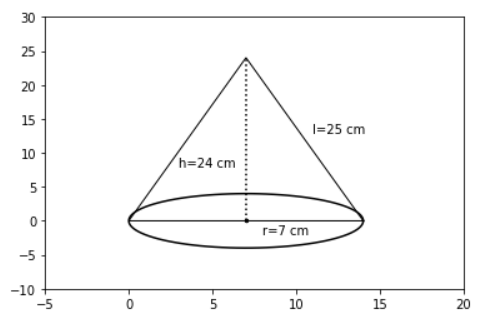
\includegraphics[width=\columnwidth]{Figs/cone.png}
	  \caption{Tent in the shape of cone}
  \end{figure}
  \section*{Steps for generating the figure}
   \begin{enumerate}
     \item First construct a isosceles triangle taking length of base as $14m$ and height of triangle as $24m$.
     \item Then,construct a ellipse taking center at midpoint of base of triangle.
     \item Taking semi-major axis length $7m$ and semi-minor axis length $4m$ for ellipse.
     \item To indicate height of cone construct a dotted line which is median of triangle and indicate other dimensions also.
   \end{enumerate} 
  
  We know that lateral/curved surface area $s$ of a cone is given
  by,
  \begin{align}
    \hspace*{12pt} s = \pi \times r \times l \\
    \Rightarrow  s = \frac{22}{7} \times 7 \times 25  \\
    \Rightarrow  s = 550 m^2 
  \end{align}
   
  Hence the curved surface area is $ 550 m^2 $. \\\\
 
 
\end{document}
